\documentclass{scrartcl}
\usepackage[utf8]{inputenc}
\usepackage[english]{babel}
\usepackage{listings}
\usepackage{graphicx}

\title{Exercise 4}
\subtitle{Data Mining Algorithms 1 - WS 2015/16}
\author{
  Davide Pedranz\\ \texttt{(362504)}
  \and
  Jakub Amanowicz \\ \texttt{(362594)}
  \and
  Hongmei Liang\\  \texttt{(292520)}
}

\usepackage{Sweave}
\begin{document}
\input{4.5-concordance}
\section*{Exercise 4.5}

\subsection*{Code}
\lstinputlisting[language=R, breaklines=true]{4.5.R}

\bigskip
\bigskip

\subsection*{Output}
\begin{Schunk}
\begin{Soutput}
Apriori

Parameter specification:
 confidence minval smax arem  aval originalSupport support minlen maxlen
        0.8    0.1    1 none FALSE            TRUE    0.05      1     10
            target   ext
 frequent itemsets FALSE

Algorithmic control:
 filter tree heap memopt load sort verbose
    0.1 TRUE TRUE  FALSE TRUE    2    TRUE

Absolute minimum support count: 491 

set item appearances ...[0 item(s)] done [0.00s].
set transactions ...[169 item(s), 9835 transaction(s)] done [0.00s].
sorting and recoding items ... [28 item(s)] done [0.00s].
creating transaction tree ... done [0.00s].
checking subsets of size 1 2 done [0.00s].
writing ... [31 set(s)] done [0.00s].
creating S4 object  ... done [0.00s].
\end{Soutput}
\begin{Soutput}
   items                         support   
28 {whole milk}                  0.25551601
27 {other vegetables}            0.19349263
26 {rolls/buns}                  0.18393493
24 {soda}                        0.17437722
25 {yogurt}                      0.13950178
21 {bottled water}               0.11052364
23 {root vegetables}             0.10899847
22 {tropical fruit}              0.10493137
19 {shopping bags}               0.09852567
20 {sausage}                     0.09395018
17 {pastry}                      0.08896797
18 {citrus fruit}                0.08276563
8  {bottled beer}                0.08052872
12 {newspapers}                  0.07981698
1  {canned beer}                 0.07768175
16 {pip fruit}                   0.07564820
31 {other vegetables,whole milk} 0.07483477
14 {fruit/vegetable juice}       0.07229283
15 {whipped/sour cream}          0.07168277
9  {brown bread}                 0.06487036
13 {domestic eggs}               0.06344687
7  {frankfurter}                 0.05897306
10 {margarine}                   0.05856634
2  {coffee}                      0.05805796
6  {pork}                        0.05765125
30 {whole milk,rolls/buns}       0.05663447
29 {whole milk,yogurt}           0.05602440
11 {butter}                      0.05541434
4  {curd}                        0.05327911
3  {beef}                        0.05246568
5  {napkins}                     0.05236401
\end{Soutput}
\begin{Soutput}
Apriori

Parameter specification:
 confidence minval smax arem  aval originalSupport support minlen maxlen target
        0.7    0.1    1 none FALSE            TRUE   0.004      2     10  rules
   ext
 FALSE

Algorithmic control:
 filter tree heap memopt load sort verbose
    0.1 TRUE TRUE  FALSE TRUE    2    TRUE

Absolute minimum support count: 39 

set item appearances ...[0 item(s)] done [0.00s].
set transactions ...[169 item(s), 9835 transaction(s)] done [0.00s].
sorting and recoding items ... [126 item(s)] done [0.00s].
creating transaction tree ... done [0.00s].
checking subsets of size 1 2 3 4 5 done [0.00s].
writing ... [5 rule(s)] done [0.00s].
creating S4 object  ... done [0.00s].
\end{Soutput}
\begin{Soutput}
  lhs                     rhs                    support confidence     lift
1 {tropical fruit,                                                          
   root vegetables,                                                         
   yogurt}             => {whole milk}       0.005693950  0.7000000 2.739554
2 {butter,                                                                  
   curd}               => {whole milk}       0.004880529  0.7164179 2.803808
3 {curd,                                                                    
   domestic eggs}      => {whole milk}       0.004778851  0.7343750 2.874086
4 {citrus fruit,                                                            
   tropical fruit,                                                          
   root vegetables}    => {other vegetables} 0.004473818  0.7857143 4.060694
5 {tropical fruit,                                                          
   yogurt,                                                                  
   whipped/sour cream} => {whole milk}       0.004372140  0.7049180 2.758802
\end{Soutput}
\end{Schunk}

\subsection*{Graph}
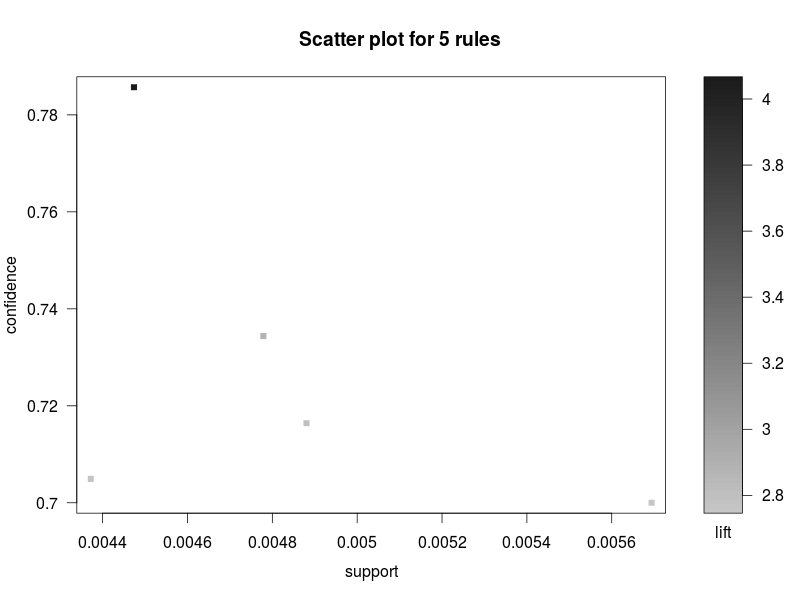
\includegraphics[width=\textwidth]{plot.png}

\bigskip

An interesting rule found is the following (with the highest confidence):
$$\{citrus fruit, tropical fruit, root vegetables\} \Rightarrow \{other vegetables\}$$

\end{document}
